Neste teste foi medido o tempo gasto com a gera��o de terrenos tanto na \emph{GPU} quanto na \emph{CPU}. Para cada n�mero de \emph{octaves} (4, 8, 12, 16), foi gerado 100 terrenos, e medido o tempo gasto. Quaisquer outros par�metros (n�mero de v�rtices, tamanho de texturas, n�meros de vizinhos) foram mantidos iguais para a gera��o nas duas arquiteturas. Os resultados obtidos est�o na tabela \ref{tabela:geracao}.


\begin{table}[H]
	\begin{center}
		\begin{tabular}{|c|c|c|}
			\hline
			\emph{Octaves} & GPU & CPU \\
			\hline
			4 & 28,7236 & 46,2948\\
			\hline
			8 & 28,7432 & 92,4299\\
			\hline
			16 & 28,7887 & 187,103\\
			\hline
			32 & 30,1095 & 370,841\\
			\hline
		\end{tabular}
		\caption{Tempo m�dia (em ms) de gera��o dos terrenos, com n�mero vari�vel de \emph{octaves}}
		\label{tabela:geracao}
	\end{center}
\end{table}


A Figura \ref{fig:geracao} apresenta os tempos anteriores.
\begin{figure}[H]
	\center{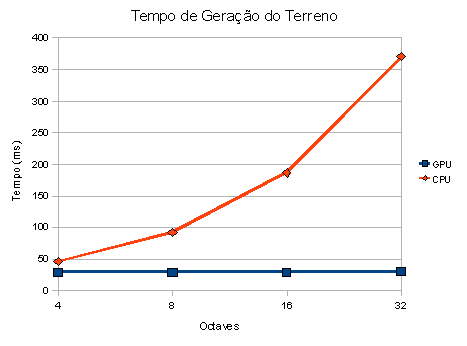
\includegraphics[width=0.5\linewidth]{img/tempoGeracao.png}}
	\caption{\label{fig:geracao} Gr�fico do tempo m�dio (em ms) de gera��o dos terrenos, com n�mero vari�vel de \emph{octaves}.}
\end{figure}

